\documentclass[a4paper,11pt,UTF8]{article}
\usepackage{ctex}
\usepackage{amsmath,amsthm,amssymb,amsfonts}
\usepackage{amsmath}
\usepackage[a4paper]{geometry}
\usepackage{graphicx}
\usepackage{microtype}
\usepackage{siunitx}
\usepackage{booktabs}
\usepackage[colorlinks=false, pdfborder={0 0 0}]{hyperref}
\usepackage{cleveref}
\usepackage{esint} 
\usepackage{graphicx}
\usepackage{ragged2e}
\usepackage{pifont}
\usepackage{extarrows}
\usepackage{mathptmx}
\usepackage{float}
\usepackage{caption}
\captionsetup[figure]{name={Figure}}

\title{Microelectronics Circuit Analysis and Design Homework(6th)}
\author{Yuejin Xie \quad U202210333}
\date{Sept 27th, 2023}
\begin{document}
\maketitle
\noindent4.15 For the NMOS common-source amplifier in Figure P4.15, the transistor
parameters are: $V_{T N }= 0.8$V, $K_n = 1\text{mA/V}^2$, and $\lambda = 0$. The circuit parameters
are $V_{DD} = 5 $V, $R_S = 1 k\Omega$, $R_D = 4 k\Omega$, $R_1 = 225 k\Omega$, and
$R_2 = 175 k\Omega$. (a) Calculate the quiescent values $I_{DQ}$ and $V_{DSQ}$. (b) Determine
the small-signal voltage gain for $R_L =\infty$. (c) Determine the value of
$R_L$ that will reduce the small-signal voltage gain to 75 percent of the value
found in` part (b).\\
\begin{figure}[H] 
	\centering 
	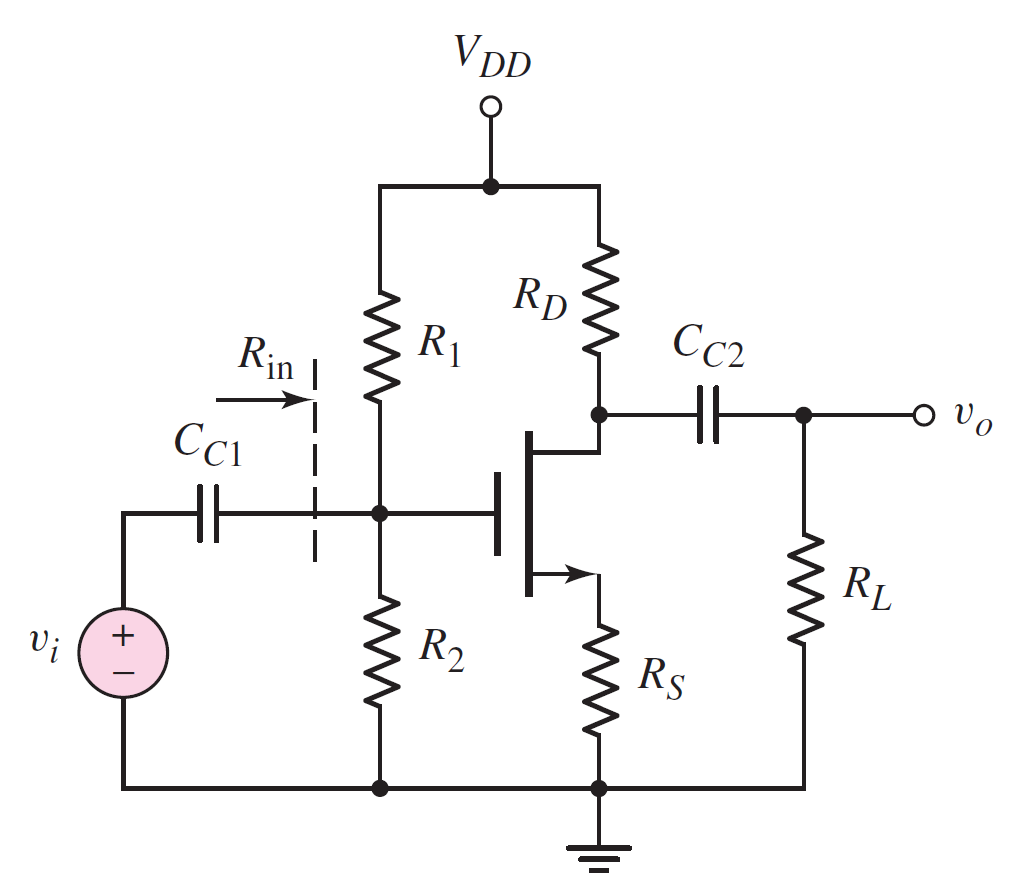
\includegraphics[scale=0.3]{MD4.15.png}
	\caption{Problem 4.15/4.17}
\end{figure}
\noindent Solution:\\
(a)$\displaystyle V_{G}=\frac{R_2}{R_1+R_2}V_{DD}=\frac{35}{16}$V, assume that the transistor work in the saturation region:\\
$V_{S}=I_DR_S, I_D=K_n(V_G-V_S-V_{TN})^2\Rightarrow I_D=0.61\text{mA or }3.17\text{mA}(Ignore)$\\
$\therefore V_{GS}=V_G-V_S=1.58\mathrm{V}V_{DSQ}=V_{DD}-I_DR_D=1.96\mathrm{V}>V_{GS}-V_{TN}$\\
(b)$R_L=\infty \Leftrightarrow$ Circuit is open, so the equivalent circuit is as follow:\\
\begin{figure}[H] 
	\centering 
	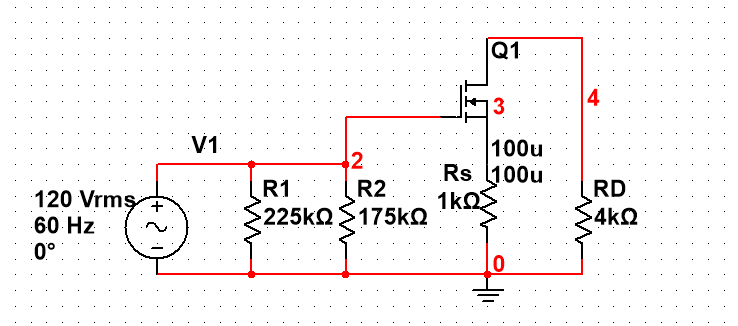
\includegraphics[scale=0.5]{MD4.15_1.png}
	\caption{Problem 4.15}
\end{figure}
\noindent$\displaystyle g_m=2K_n(V_{GSQ}-V_TN)=1,56\mathrm{mS}, i_d=g_mv_{gs},v_o=-i_dR_D, A_v=\frac{v_o}{v_{gs}}=-2.44$\\
(c)$\displaystyle A_v^\prime=0.75A_v=\frac{-i_d(RL||R_D)}{v_{gs}}\Rightarrow R_L=12\mathrm{k}\Omega$\\
4.17 Repeat Problem 4.15 if the source resistor is bypassed by a source capacitor
$C_S$.\\
(a)The answer is the same as 4.15(a), because in the case of DC, the source capacitor is open, answer doesn't change.\\
$I_D=0.61\mathrm{mA},V_{DSQ}=1.96\mathrm{V}$\\
(b)(c)In this case, the $R_S$ is shorted, but $i_d$ doesn't change, so the answer is the same as 4.15(b)(c)\\
$\therefore$(b)$\displaystyle A_v=-2.44$ (c)$R_L=12\mathrm{k}\Omega$\\
D4.26 Design the common-source circuit in Figure P4.26 using an n-channel
MOSFET with $\lambda = 0$. The quiescent values are to be $I_{DQ} = 6 $mA,
$V_{GSQ} = 2.8$ V, and $V_{DSQ} = $10 V. The transconductance is $g_m = 2.2 $mA/V.
Let $R_L = 1 k\Omega$, $A_v = -1$, and $R_{in} = 100 k\Omega$. Find $R_1, R_2, R_S, R_D, K_n$, and $V_{T N}$ .\\
\begin{figure}[H] 
	\centering 
	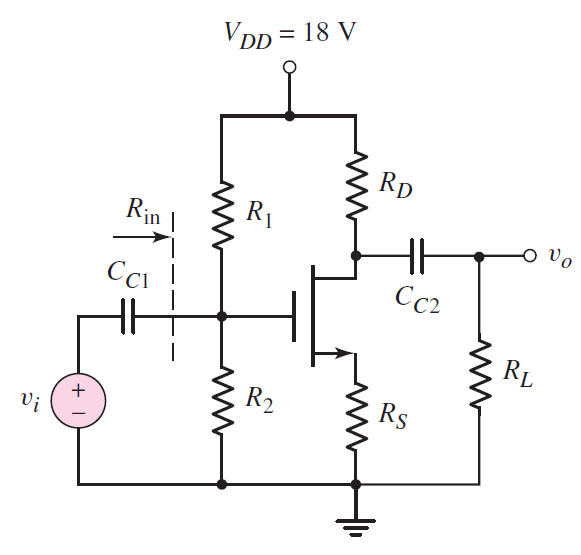
\includegraphics[scale=0.5]{MD4.26.png}
	\caption{Problem 4.26}
\end{figure}
\noindent Solution:\\
Obviously, the transistor is work in the saturation region, we have equation:\\
$$\begin{cases}\displaystyle
	I_{DQ}=K_n(V_{GSQ}-V_{TN})^2\\
	V_{DSQ}=V_{DD}-I_DR_D\\
	\displaystyle V_G=\frac{R_2}{R_1+R_2}V_{DD}\\
	V_S=I_DR_S\\
	g_m=2K_n(V_{GSQ}-V_{TN})\\
	\displaystyle R_{in}=\frac{R_1R_2}{R_1+R_2}\\
	\displaystyle A_v=\frac{-g_mv_{gs}(R_D||R_L)}{v_{gs}}
\end{cases}\Rightarrow
\begin{cases}
	R_1=\\
	R_2=\\
	R_S=\\
	R_D=\\
	K_n=\\
	V_{T N}=\\
\end{cases}$$
\end{document}